\section{Virtualization Overview}

\subsection{Motivation}

I can hardly say enough about virtualization.  It's pervasiveness and
impact on the IT world can hardly be overstated.  Also, IT
environments are getting more and more complicated and having a
wholistic understanding of the whole topology begins to get too
complicated.  We have experts in fields of a given domain who have
trouble communicating with each other.  It's my assertion that every
member of the IT team should be able to install all the key pieces of
their organizations infrastruture so they can test the effects of
making changes etc.  When you use a Virtual infrastructure to do this,
you can set it up and tear it down without worring about having to buy
a whole lot of hardware.

Organization that can understand the value of this will make huge
strides in taming the wild animal of their infrastructure and begin to
create much better infrastructures.  So lets roll up our sleeves and
come to understand about the types of virtualization so we can get
busy using it.
	
\begin{figure}[h!]
  \centering
  \fbox{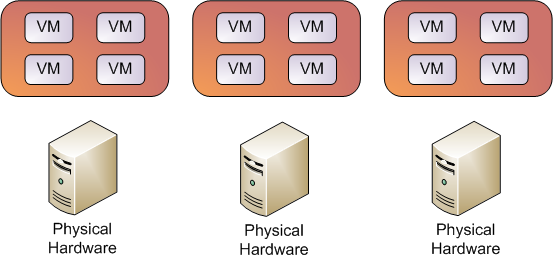
\includegraphics[width=130mm]{images/VirtualMachines}}
  \caption{Virtual Machines}
\end{figure}

\subsection{Overview}
	
Virtualization comes in two primary forms.  The type that runs on your
personal laptop, that Sales people take out to demonstrate software to
customers, and the type that runs in the back office data
centers...the 'real' virtualization.

These two type have names.  The one you run on your lap top is called
'Fully Virtualized' virtualization.  The one that runs in the data
centers is called 'Para-Virtualized'
	
If you have some familiarity with virtualization you'll probably be
familiar with fully hosted virtualization.  Products like virtual-box,
VM Ware Workstation (Player), etc... fall into this camp.  Datacenter,
para-virtualized (PV), products are VM Ware ESXi, and XEN.  There are
many many more but we'll focus mainly on Oracle Virtualization which
is based on XEN.
	
\begin{figure}[h!]
  \centering
  \fbox{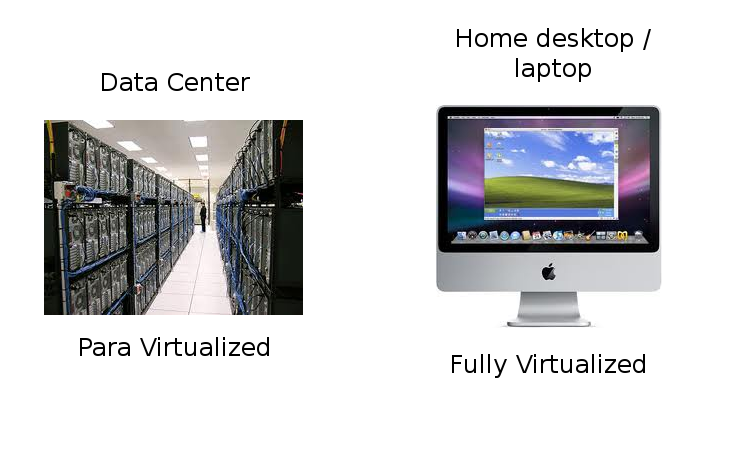
\includegraphics[width=130mm]{images/paraVsFullyVirtualized}}
  \caption{Para versus Fully virtualized}
\end{figure}

\subsection{Whats appropriate for you?}

When deciding which route you want to go, you will for sure want to
become familiar with fully virtualized solutions, such as Virtual Box.
The reason for this is that it is simple to setup and use on the
operating system you currently have.  They will all support Windows,
Linux or Mac OS's.
	
I would highly recommend that you also try to do PV virtualization as
well, since if you want to run this in production that is the way you
would go.  You need to have dedicated hardware for this.  A spare
laptop will do, and having the maximum amount of RAM is also highly
recommended.